%% ---------------------------------------------------------------------------------------------------------
\section{Introduction}\label{sec:intro}

Learned visuomotor policies such as diffusion policies \cite{chi2023diffusion} are increasingly deployed as frozen components: after training, their weights are fixed, and any further improvement must come from outside the network. A natural outside improvement is a runtime recovery intervention: a rule or monitor decides that something is about to go wrong, a small controller changes the state, and the policy resumes. Many methods of this kind exist, from learned recovery policies \cite{reichlin2022manifold,cideron2023getback,vats2025recoverychaining} to human or learned interventions during interactive imitation \cite{ross2011dagger,kelly2019hgdagger,hoque2022thrifty}, and runtime monitors that detect or predict failures \cite{agia2025unpacking,romer2025fiper,liu2023reflect,duan2025aha}.

\paragraph{Why harm must be measured separately}
An intervention on a frozen policy changes the state from which the policy continues. If the policy would have failed, the change can rescue the episode. If the policy would have succeeded, the same change can cause a failure, for example by spending part of the time budget or by leaving the gripper in a configuration from which the policy does not recover. On $n$ paired scenes with $R$ rescues and $H$ harms, the change in success rate is
\begin{equation}\label{eq:delta}
\Delta_{\mathrm{succ}} \;=\; \frac{R-H}{n}.
\end{equation}
Two interventions with $(R,H)=(30,0)$ and $(60,30)$ have the same $\Delta_{\mathrm{succ}}$, but the second loses 30 episodes that the user could previously rely on. A success rate, or a comparison of success rates measured on different scenes, cannot distinguish them; only a paired comparison on the same states can. Harm therefore needs its own measurement and, if an intervention is to be deployed on top of a policy that already works most of the time, its own bound.

\begin{figure}[!htbp]
\centering
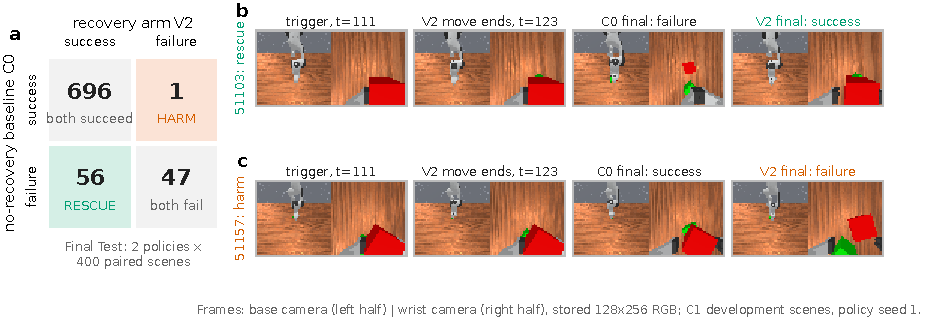
\includegraphics[width=\linewidth]{Fig01_problem_rescue_vs_harm.pdf}
\caption{Rescue and harm. (a) Paired outcome matrix of the Final Test, pooled over the two policies (descriptive; the tests are per policy). (b) A development rescue (scene 51103, policy seed 1; the first seed-1 rescue in scene order): the policy alone fails; after the V2 move the re-planned policy places the cube and the episode succeeds. (c) The only development harm of V2 for policy seed 1 (scene 51157): the policy alone drops the cube beside the target, regrasps it and succeeds at step 190; with V2 the episode fails. Each frame is the stored base-camera (left half) and wrist-camera (right half) RGB image, without processing or overlay.}\label{fig:problem}
\end{figure}

\paragraph{Detection is not intervention}
A failure monitor answers whether something will go wrong; it does not answer whether a particular action taken at that moment will make the outcome better or worse. The second question is counterfactual: it compares the outcome with and without the action from the same state \cite{ahmedt2026rescue}. In this paper the trigger is a fixed, observable rule, so the object of study is the intervention itself, not the detector.

\paragraph{Case study}
We study one intervention in depth: an observation-only, gated centring move at the moment a frozen diffusion policy is about to release a cube over another cube. We chose it because it can be evaluated cleanly: it acts at most once per episode, it uses only the robot's cameras and proprioception, it needs no retraining, and when it abstains the episode is exactly the uninterrupted one. The question we answer is: \emph{can such an intervention increase task success while keeping, with a finite-sample statistical guarantee, the rate at which it turns the policy's own successes into failures below a stated level?} We answer it for one task, one intervention and two independently trained policies, and we report every step of the argument, including the parts that did not work.

The study rests on three design choices.
\begin{enumerate}
\item \textbf{Paired branching.} Each scene runs once until the trigger; the simulator state is saved, and the uninterrupted policy (C0), the proposed controller and all ablations are run from that same snapshot. Each scene yields a pair of outcomes $(Y_0, Y_g)$ and falls into one of four cells: both succeed, rescue, harm, both fail (Fig.~\ref{fig:problem}a).
\item \textbf{Harm as a conditional rate.} We define harm as $h(g)=\Pr(Y_g=0 \mid Y_0=1)$, the probability that intervention $g$ turns a baseline success into a failure, and test $h(g)<\varepsilon$ against $h(g)\ge\varepsilon$ with an exact binomial test on calibration scenes that were not used for development.
\item \textbf{Separation of certificate and efficacy.} The harm certificate is computed on a calibration split; the efficacy claim (more successes than without the intervention) is tested once on a separate, held-out test split, under a frozen and hashed protocol. Development results motivate the design and are reported as such.
\end{enumerate}

\paragraph{The strongest objection, stated first}
A low harm rate can simply mean that the controller rarely acts. This is largely true here: V2 abstains in about four of five triggered scenes, and harm can only occur in scenes where it moves. Restricted to the baseline successes in which it moved, the observed harm is 1 of 48 and 0 of 36 on calibration, and the corresponding one-sided upper bounds are near 10\%, not 5\% (Section~\ref{sec:confirm}). We therefore state the certificate as a property of the deployed system, the policy together with its gated controller, and we do not claim that the abstention rules themselves reduce harm: an ablation without the V2-specific rules rescued slightly more scenes without additional harm in development (Section~\ref{sec:discussion}).

\paragraph{Contributions}
\begin{itemize}
\item A paired evaluation protocol for recovery interventions on a frozen policy that reports rescue and harm separately, certifies the conditional harm rate with a pre-registered exact test on a calibration split, and confirms efficacy once on a held-out split (Sections~\ref{sec:problem} and~\ref{sec:protocol}).
\item Vision-CENTER V2, an observation-only release-time centring controller with a confirmed visual memory and explicit abstention rules, described as implemented (Section~\ref{sec:method}).
\item A two-stage confirmatory result on 1,600 new paired scenes for two policies (Section~\ref{sec:confirm}).
\item A descriptive mechanism analysis that follows a representative rescue and the single development harm through observation, memory, decision, movement and hand-back, with a commanded-versus-actual motion audit of all development moves (Section~\ref{sec:mechanism}).
\item An audit of the physical record used by that analysis, including a pre-declared check that fails, a partial explanation of the failure, and a statement of what it does and does not affect (Section~\ref{sec:physics}).
\end{itemize}

We do not claim physical safety, transfer to other tasks or to a real robot, or novelty of paired counterfactual evaluation, of exact binomial bounds or of risk control; these are established tools \cite{clopper1934,holm1979,angelopoulos2021ltt,ahmedt2026rescue}. The contribution is their combination for a runtime recovery intervention, with a calibration/test separation and a code-level account of why the intervention rescues and how it harms. The controller is task-specific; we present it as a case study of the protocol, which is the part we expect to transfer.
